% Pascal's rule at n=3, k=2: subsets that contain a fixed element, and subsets that do not.
\begin{tikzpicture}[x=1cm,y=1cm]
  \node[anchor=west,font=\small] at (0,2.05) {the $2$-element subsets of $\{a,b,c\}$};
  \node[anchor=west,font=\scriptsize] at (0,1.45) {contain $a$};
  \draw[MidnightBlue,thick,rounded corners=2pt] (0,0.05) rectangle (2.55,1.15);
  \node[font=\small] at (1.27,0.78) {$\{a,b\}$};
  \node[font=\small] at (1.27,0.38) {$\{a,c\}$};
  \node[font=\small] at (3.05,0.60) {$+$};
  \node[anchor=west,font=\scriptsize] at (3.55,1.45) {omit $a$};
  \draw[BrickRed,thick,rounded corners=2pt] (3.55,0.05) rectangle (6.1,1.15);
  \node[font=\small] at (4.82,0.60) {$\{b,c\}$};
  \node[font=\small] at (6.55,0.60) {$=$};
  \node[anchor=west,font=\small] at (7.05,0.60) {$\dbinom{3}{2}=3$};
  \node[anchor=west,font=\scriptsize] at (0,-0.45) {$\dbinom{2}{1}$ subsets of $\{b,c\}$};
  \node[anchor=west,font=\scriptsize] at (3.55,-0.45) {$\dbinom{2}{2}$ subset};
\end{tikzpicture}
